\chapter{Stand van zaken}
\label{ch:stand-van-zaken}

% Tip: Begin elk hoofdstuk met een paragraaf inleiding die beschrijft hoe
% dit hoofdstuk past binnen het geheel van de bachelorproef. Geef in het
% bijzonder aan wat de link is met het vorige en volgende hoofdstuk.

% Pas na deze inleidende paragraaf komt de eerste sectiehoofding.
Om growth hacking te kunnen kaderen moet men begrijpen waar het begrip van komt en hoe het ontstaan is. De bron van growth hacking ligt in bij marketing, digitale marketing, influencer marketing enz. In de volgende paragrafen zullen deze begrippen duidelijk gemaakt worden en op het einde van dit hoofdstuk zal er een concrete definitie gevormd worden over growth hacking.

\section{Wat is marketing?}
\label{sec:marketing}
\begin{quote}
	``Alles wat een bedrijf doet om de verkoop van producten te bevorderen.``, definitie van marketing. \textcopyright  woorden.org
\end{quote}
Marketing kan men ook uitleggen aan de hand van de marketingmix (4 P's), die E Jerome McCarthy in 1960 ontwikkelde om marketing te verduidelijken. Deze 4 P's staan in connectie met elkaar en een aanpassing kan zorgen voor een volledig nieuwe marketing mix.~\autocite{Forsey2019}

\begin{itemize}
	\item Product
	\item Prijs
	\item Plaats
	\item Promotie
\end{itemize}

De marketingmix wordt gebruikt om het marketingbeleid van een organisatie te beschrijven. 

\subsection{Product}
\label{sec:marketing-product}
Deze eerste P duidt zowel een product als dienst aan. Een klant moet de nood of wens van een klant voldoen. Het product dient een meerwaarde te bieden voor de klant. Binnen marketing is het belangrijk om dat het product goed en volledig is. Van design tot verpakking en alle services die er bij komen.
 
\subsection{Prijs}
\label{sec:marketing-prijs}
"Wat is de prijs dat onze doelgroep wil betalen voor ons product?" is een belangrijke vraag. De juiste kostprijs bepalen zodat het bedrijf winstgevend kan zijn. Het gaat over prijsbepaling en strategie, maar ook kortingen.

Een opvallende trend in bij webshops en andere web platformen is dat er vaak korting is op veel producten. Het product is steeds goedkoper dan de ``adviesprijs``, dit is een manier om psychologische prijzen in te zetten. Een andere strategie is de prijs goedkoper te laten aanvoelen, in plaats van 10 euro kan men 9,99 vragen voor hetzelfde product~\autocite{InternetMarketingUniversiteit2016}. Dit heet ``Charm pricing``, het verschil in prijs is miniem. De consument zal eerder het product kopen dat goedkoper is dan de adviesprijs en begint met een lager getal (door de 99 cent bijvoorbeeld), dan het product dat 10 euro kost en niet goedkoper is of blijkt te zijn.

\subsection{Plaats}
\label{sec:marketing-plaats}
Plaats dient een antwoord te geven op de gehele distributie van het product. "Op welke manier komt de dienst of het product bij de klant?". 

\subsection{Promotie}
\label{sec:marketing-promotie}
Dit wordt ook wel marketingcommunicatie genoemd. Dit is waar men meestal aan denkt wanneer iemand marketing vermeld.

Promotie maken voor je product, er voor zorgen dat men weet wat je bedrijf doet of verkoopt. Ook het imago van het bedrijf is hier onderdeel van.

Enkele promostrategieën~\autocite{marketingscriptie.nl2018}:
\begin{itemize}
	\item Reclame (internet, krant, televisie)
	\item Public Relations (bijvoorbeeld sponsoring)
	\item Plaats (acties)
	\item Persoonlijke verkoop (face-to-face, telefonisch, ...)
\end{itemize}

\section{Invloed van de digitalisering op marketing}
\label{sec:digitalisering-marketing}
De digitalisering heeft een grote invloed gehad op de manier waarop bedrijven aan marketing doen. Een nieuwe "soort" marketing is ontstaan: digitale marketing. 

Hiervoor bestaan nu ook nieuwe jobs, de all-around digital marketeer kan op z'n eentje de marketing doen van een klein bedrijf. Grote bedrijven hebben vaak een specialist in SEO, die zorgt ervoor dat de website van het bedrijf makkelijk gevonden kan worden via populaire zoekmachines zoals Google en Bing. Naast een SEO specialist bestaat er vaak een community manager die via sociale media contact direct heeft met de klanten. Google en Facebook advertising kunnen door aparte teams onderhouden worden. Verder bestaan er ook "lead generator"-experts, die via verschillende regels de ideale manier kunnen vinden om potentiële klanten binnen te halen.

\section{Nieuwe trends binnen marketing}
\label{sec:nieuwe-trends-marketing}
Nu dat digitale marketing een zekere maturiteit heeft en dat zo wat alle grote bedrijven aan digitale marketing doen, ontstaan er natuurlijk nieuwe trends. 

\subsection{Influencer marketing}
\label{sec:influencer-marketing}
Influencer marketing is hier één van. Zoals~\textcite{Pieters2018} aangeeft in zijn bachelorproef~\citetitle{Oord2014} is Instagram een populair en efficiënt platform om aan influencer marketing te doen. 

Een influencer is een persoon of groep personen die een meer dan gemiddeld potentieel hebben om anderen te beïnvloeden doordat zij veel communiceren en zich centraal bevinden in een (sociaal) netwerk.~\autocite{Pieters2018}

Bedrijven kunnen deals sluiten met influencers zodat ze het product of de service van het bedrijf promoten, bijvoorbeeld via een post op Instagram. Dit is veel persoonlijker dan een generieke advertentie via een digitaal medium zoals Google Adwords, Facebook Ads (hier hoort Instagram ook bij) of dergelijke. Vaak hebben influencers een bepaalde doelgroep, wanneer deze perfect aansluit bij het bedrijf zal het product waarschijnlijk ook goed ontvangen worden door de volgers van de influencer. Hierdoor kan één post een heel positieve impact hebben op de omzet van het bedrijf. De influencer wordt vaak vergoed door een geldsom, soms kan dit ook een verblijf in het buitenland zijn voor bepaalde activiteiten. Door het bedrijf wordt de reis, het verblijf en de activiteiten dan betaald. Beide partijen komen er op deze manier beter uit.


\subsection{Content marketing}
\label{sec:content-marketing}
Content marketing is een belangrijk fenomeen in de digitale marketing wereld. Het behalen van een goede score bij zoekmachines ligt voor een groot deel bij het schrijven van goede content. Bij het schrijven van deze 'goede content' moet er steeds rekening gehouden worden met de belangrijke keywords die rond het onderwerp vaak gezocht worden. 

In 2014 schreef Bob Oord van RIFF Content Marketing over thesis~\citetitle{Oord2014}. In dit artikel bespreekt hij de verschillende rollen die de marketingafdeling in 2020 zou bevatten. Hij spreekt over heel veel rollen, maar deze kunnen ondergebracht worden onder enkele functies of binnen een klein bedrijf 1 functie: de contentmarketeer. 

\subsection{Guerrillamarketing}
\label{sec:guerrillamarketing}
Guerillamarketing wordt vaak samen gebruikt met "Zero Budget Marketing" en growth hacking. Het is een marketingtechniek waarbij men met beperkte middelen een groot resultaat wil behalen. De focus ligt op het halen van veel (media-)aandacht tot het merk of product. Men wil een groot publiek bereiken en er voor op die manier voor zorgen dat het publiek vertrouwd geraakt met de merknaam of het product.

Dit gebeurt door bijvoorbeeld ludieke acties of stunts die heel snel en efficiënt zijn in het bereiken van een groot publiek. 

Growth hacking kan men onder de term Guerillamarketing plaatsen, want in essentie wil men via growth hacking ook met beperkte middelen een groot resultaat behalen.

Enkele voorbeelden van gueriallamarketing:
 
\begin{itemize}
	\item Reverse graffiti: selectief schoon maken van een muur 
	\item Virale marketing: posts delen via sociale media die de ontvangers opnieuw gedeeld worden
	\item Internetmemes: door het creëren van een grappige afbeelding of post op sociale media kan deze viraal gaan
	\item Flashmob: op een openbare plek een (grote) groep mensen laten samenkomen en iets ongebruikelijks laten uitvoeren dat achteraf weer snel uiteenvalt
	\item Posters plakken: soms op illegale plaatsen, om extra aandacht te trekken
\end{itemize}

\begin{figure}[h!]
	
\includegraphics[width=150mm]{img/reverse-graffiti.jpg}
	\centering
	\caption{Reverse graffiti. \textcopyright  Lisa Müllerauh}
	\label{fig:defGrowthHacker}
\end{figure}

\begin{figure}[h!]
	
\includegraphics[width=130mm]{img/dbrand-internetmeme.jpg}
	\centering
	\caption{Internetmeme van dbrand. Ze spelen in op een recent memeformaat en passen het toe op hun eigen product(en). Zo kunnen ze met amper budget, enkel owned en earned media, een heel groot publiek laten weten dat hun product bestaat.}
	\label{fig:defGrowthHacker}
\end{figure}

\section{Wat is growth hacking?}
\label{sec:wat-is-growth-hacking}
Growth hacking is ook een nieuwe trend binnen marketing die vaak onduidelijk met zich mee brengt. Dus dan komt de vraag: wat is growth hacking nu exact?

Nicholas D’hondt beschrijft growth hacking in een artikel van~\textcite{Birdhouse2019} als een mindset van heel veel experimenteren en constant op zoek gaan naar nieuwe kanalen. 

Het gaat om zoveel mogelijk mensen binnen je doelgroep te bereiken, zo kan je als bedrijf met (zeer) weinig geld een groot resultaat behalen. 

Sommige bedrijven willen een bepaalde boodschap verspreiden, andere willen enkel hun merknaam naar buiten krijgen. Het draait steeds groeien, in welk specifiek gebied dat je wil groeien moet je voor ieder experiment steeds definiëren. Zo kan je leren uit het experiment, het is namelijk niet de bedoeling dat er zomaar uit het niets wordt geëxperimenteerd. Er zullen veel experimenten falen en het is de bedoeling dat er steeds iets uit geleerd kan worden. Dit is mogelijk door op voorhand goed te weten wat het doel is, ook moet er achteraf genoeg documentatie voorzien worden van het experiment. Waarom het doel al dan niet behaald werd kan veel verduidelijking geven en kan je in de juiste richting duwen

\subsection{Growth hacking binnen een bedrijf}
\label{sec:growth-hacker-functie}
Een growth hacker is half marketeer en half ingenieur, zoals vermeld in het onderzoeksvoorstel en geïllustreerd door de afbeelding hieronder.
\begin{figure}[h!]
	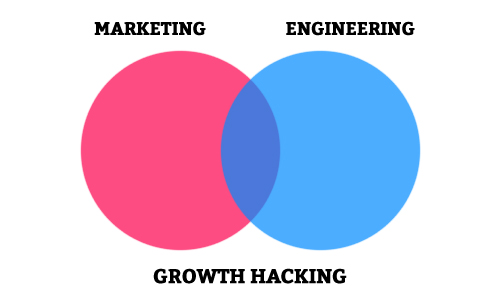
\includegraphics[width=150mm]{img/growth-hacker-definition.jpg}
	\centering
	\caption{Definitie van growth hacking, "Growth hacking as a fusion of two fields"  (Brody 2013, geciteerd 13.05.2016)}
	\label{fig:defGrowthHacker}
\end{figure}

In het artikel van The Birdhouse,~\citetitle{Birdhouse2019}, verteld Nicholas dat growth hacking moet leven in de hele organisatie. Er moet een team gecreëerd worden met mensen uit verschillende branches van het bedrijf: developers, entrepreneurs, marketing en sales zetten we bij elkaar. In deze situatie is er niet één growth hacker, er kan wel iemand zijn die alle mensen bij elkaar brengt en het concept van growth hacking uitlegt. Als we die persoon als growth hacker zien is hij of zij eerder een soort coach die het team zal helpen om rond growth hacking te brainstormen.

Bij kleinere bedrijven kan het zijn dat er één growth hacker is, deze zal dan het profiel hebben van een marketeer en ingenieur en zal doorheen het bedrijf informatie moeten vergaren. Met al die informatie kan hij of zij experimenten bedenken of collega's aanspreken en hun ideeën implementeren of deze verwerken en doorgeven aan de developers of andere marketeers. 


\section{Wat is het verschil met guerrillamarketing?}
\label{sec:verschil-met-guerrillamarketing}

info uit podcast van fizzle.co
~\citetitle{fizzle.co2015}~\autocite{fizzle.co2015}
 -- -- -- 

Guerillamarketing: old-school
- (Tactiek binnen growth hacking?): vb fysiek op een bepaalde plaats flyers uitdelen of het product verkopen (soort van stunts), graffiti, ...

Growth hacking: nieuwe buzz-worthy term
- best -> Creativiteit, want geen budget, probeer het product "out there" krijgen zonder geld
- worst -> hacking the system, no long-term solution
- don't trust it: internet markety thing
- scalable: get users to get more users. Vb: Groupon. Get people to be obsessed: viral factor. Zorg dat mensen heel tevreden zijn van het product, laat hen het verspreiden
- De aanpak van een ingenieur voor marketing : data-driven (met iteraties, opnieuw en opnieuw) experimenten
- Veel feedback vragen: maak het product samen met de klanten
- Een doel zetten: kleinere doelen hebben een groot effect (mentaal) --> zorgt voor momentum. een S.M.A.R.T. goal
- Welke marketing-kanalen kunnen we gebruiken?
- Vb.: Eerst een audience opbouwen en daarna je brand er aan koppelen (via bvb Instagram). Voorbeeld: @portland en portlandgear.
- Het gaat niet altijd plots en heel snel, vaak moet je bijvoorbeeld er heel veel tijd in steken om een bepaald aantal echte volgers te halen op Instagram. 
- growth hacking = analytical mind, get data, samenwerken met ideeën van marketeers en de confirmeren van goede of slechte ideeën
- Welke data? Wie willen we bereiken? Waar vinden we deze personas? Werkt dit experiment? Welk kanaal gebruiken we best? Komen er meer bezoekers? Meer omzet? Wordt het product aangeraden aan vrienden zoals "hebben jullie hier al van gehoord, WANT x en y"?, enz.


Er is een build-in expiration date:
- vb: FB is nu zo groot en het kost veel meer geld, vroeger was het goed als "growth hack", nu is het duur voor de keywords die je nodig hebt

